\clearpage
\section*{Question 6}
\addcontentsline{toc}{section}{Question 6}

Use any one of the fixed-time-step solvers of your own choice. Plot the solution for $i_L$ and $v_C$. Experimentally establish the largest time step $h_{\max}$ that produces a stable and convergent solution that you can trust. Compare your result with the result of using the ode5 at $h=0.5\times10^{-3}$~s and $h=1.0\times10^{-3}$~s.

\subsection*{Simulation Results}
The following figures show the results of the fixed-step simulations:
\begin{figure}[H]
	\centering
	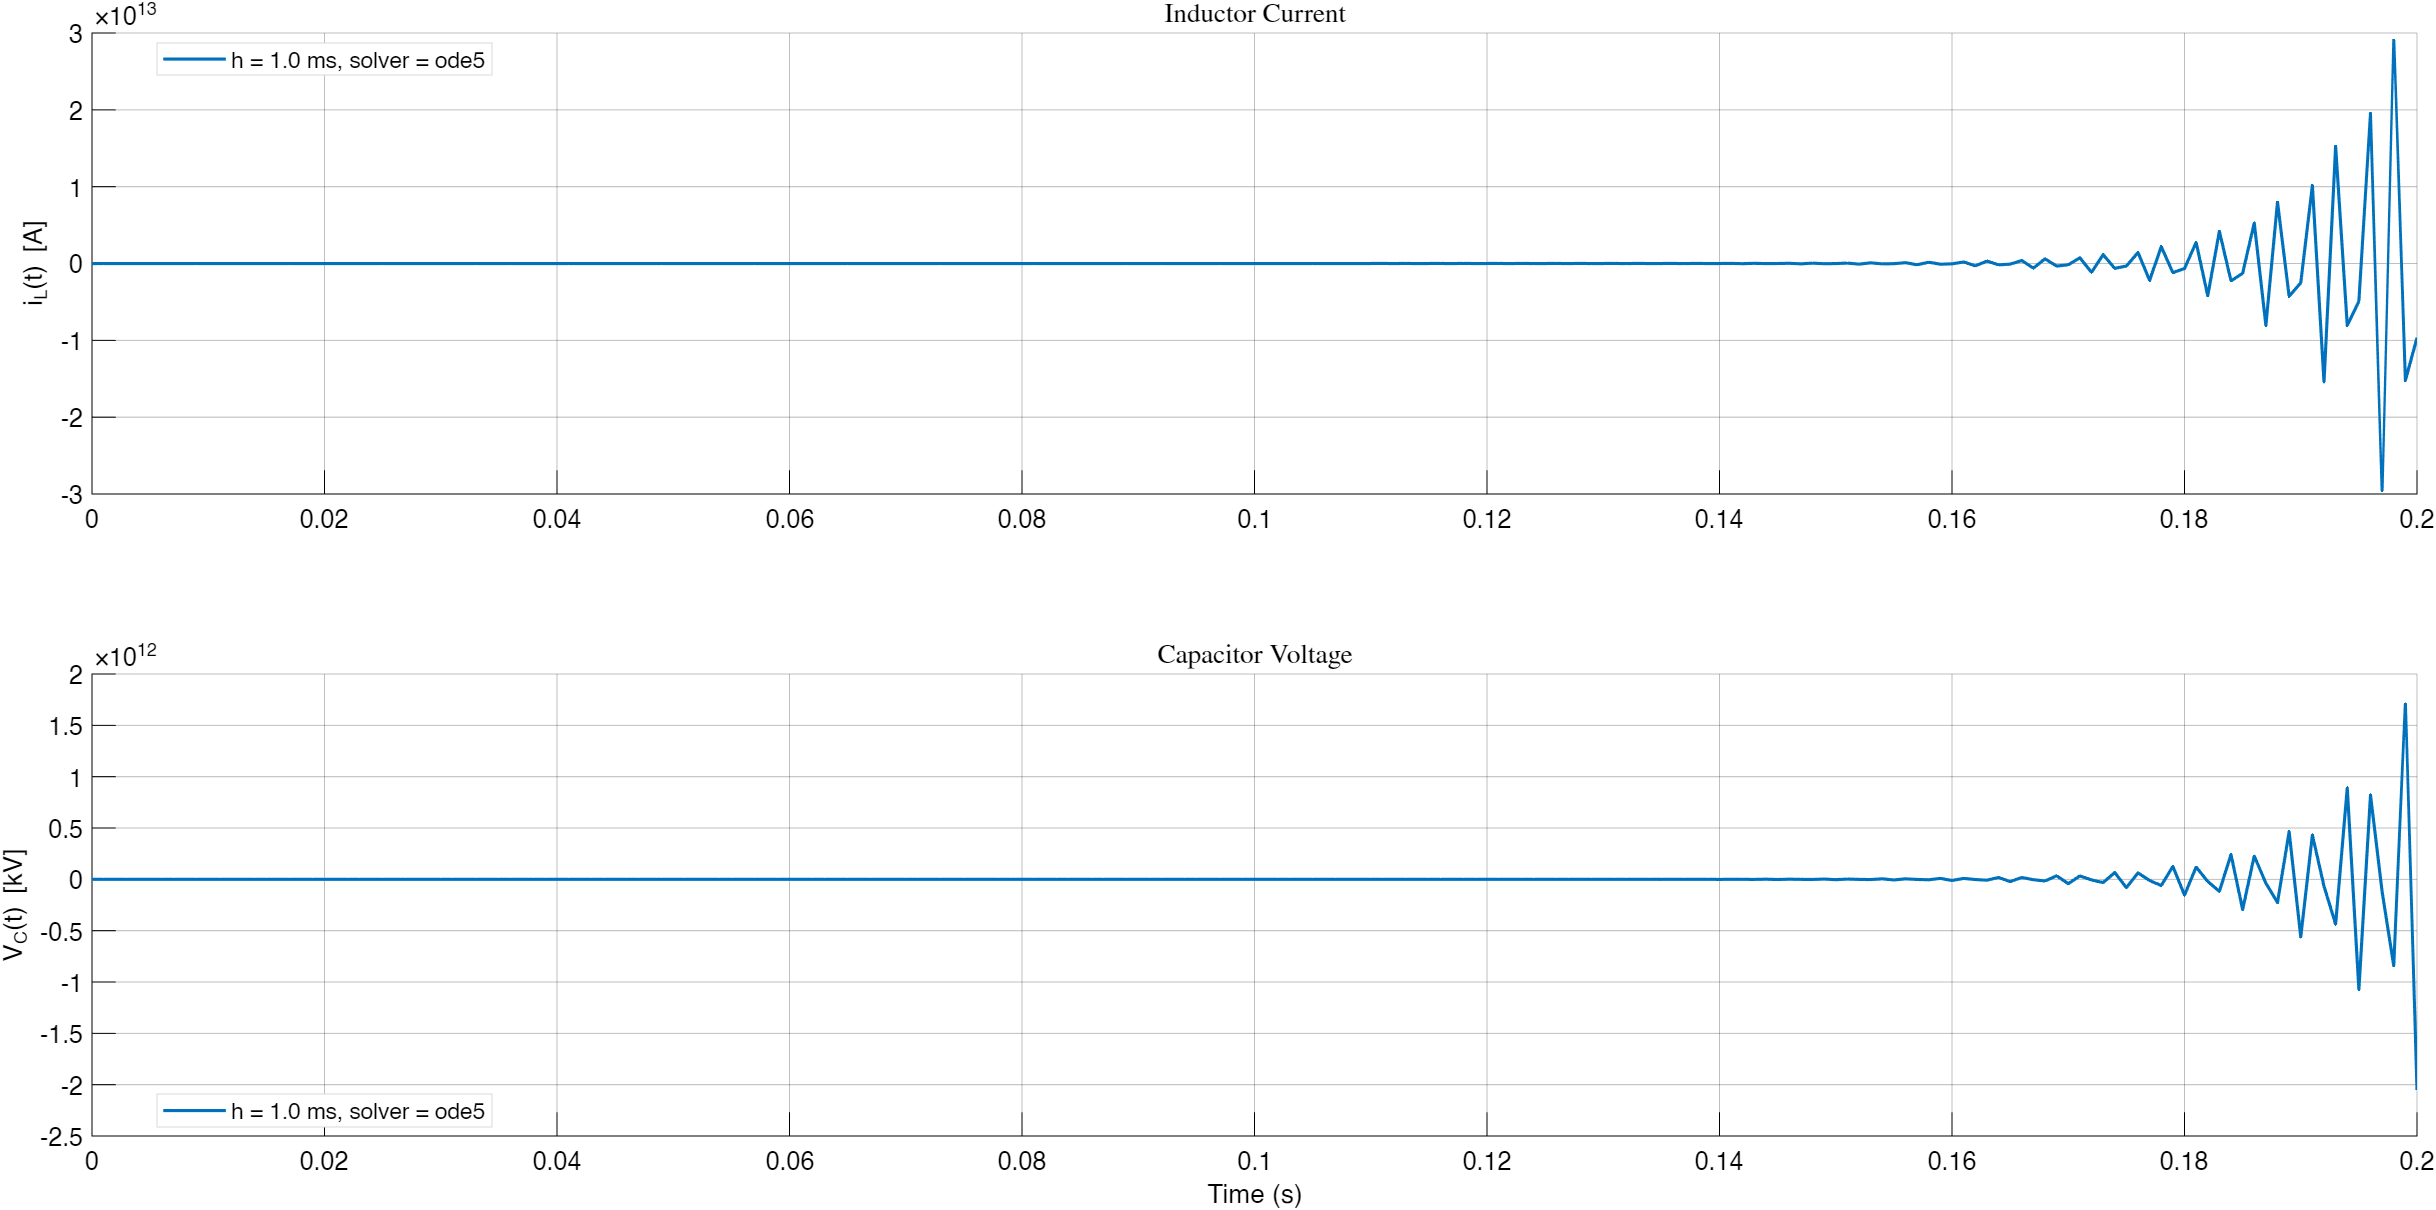
\includegraphics[width=0.95\textwidth]{figures/hw01_q06_plots-of-iL-and-Vc-for-different-ode-solvers-and-time-steps-diverging-only.png}
	\caption{Diverging solution for $h=1$ ms using ode5 (RK5).}
\end{figure}

\begin{figure}[H]
	\centering
	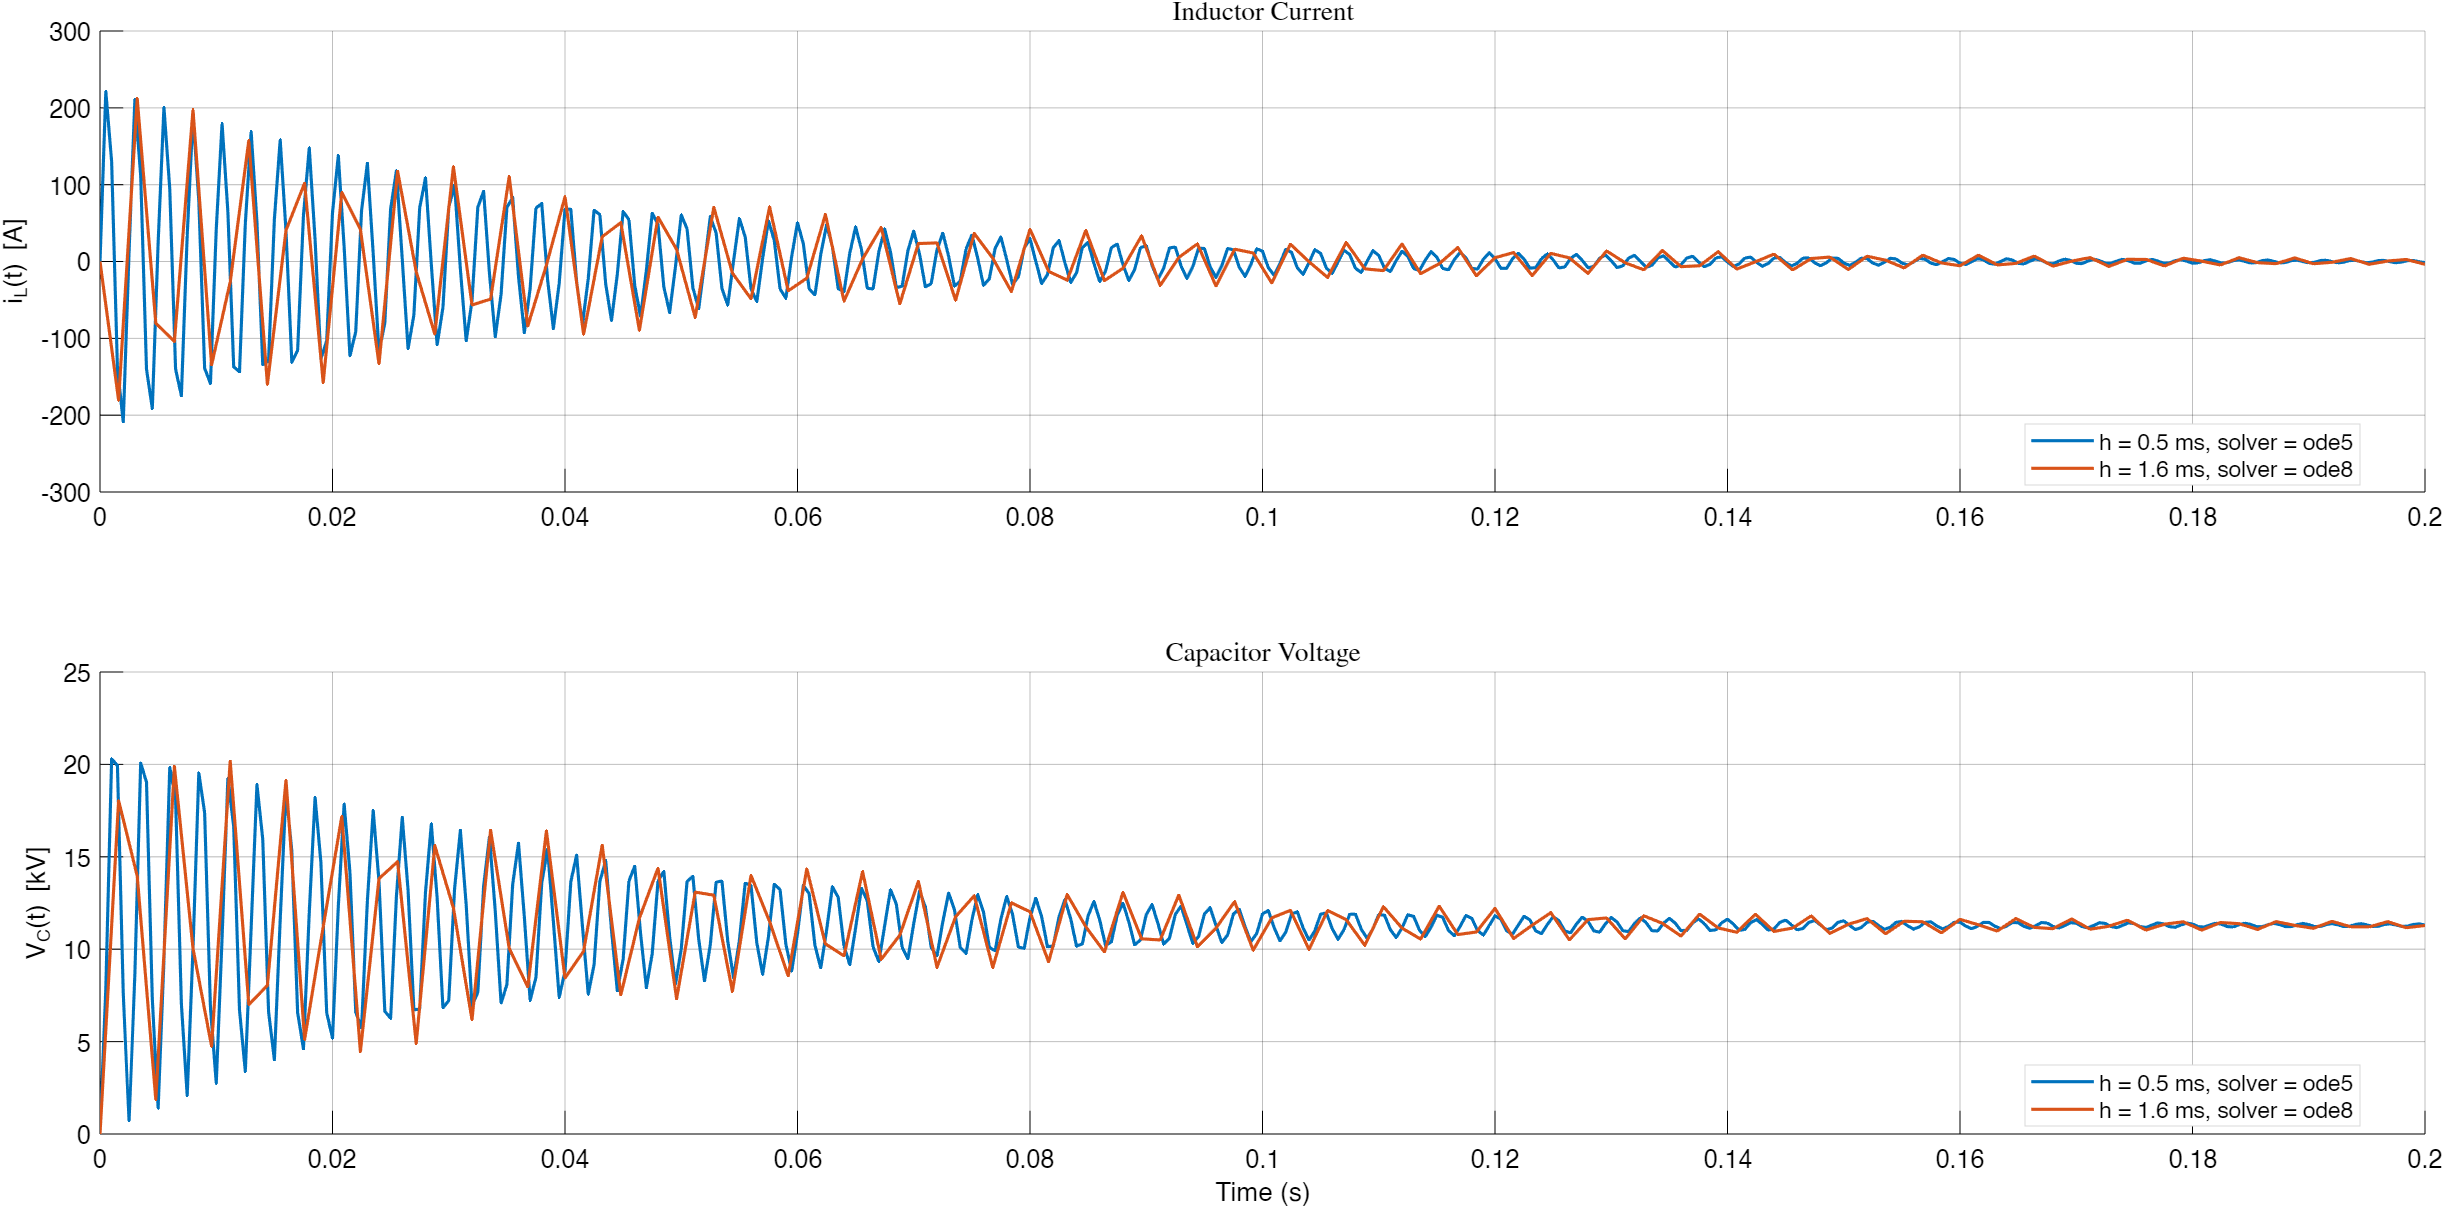
\includegraphics[width=0.95\textwidth]{figures/hw01_q06_plots-of-iL-and-Vc-for-different-ode-solvers-and-time-steps-converging-only.png}
	\caption{Converging solutions for RK8 with $h=1.6$ ms and ode5 with $h=0.5$ ms. The legend indicates the solver and step size.}
\end{figure}

\subsection*{Discussion}
For this part, I used an explicit RK8 method for my own solver. The maximum time step $h_{\max}$ for which the RK8 method produced a stable and accurate solution was determined experimentally to be $1.6$ ms. For ode5 (RK5), the $h=1$ ms case is shown separately above, as it diverges and would spoil the scale of the converging plot.

The experimentally obtained $h_{\max}$ for RK8 was found to be less than the theoretical value for Taylor-5 ($\approx 1.3$ ms). For ode5 (RK5), the maximum stable $h$ was found to be less than $0.7$ ms (figure not shown here), which is also less than the theoretical prediction. The theoretical values are based on the Taylor-5 stability region, but ode5 is not exactly Taylor-5, and RK8 has a different (larger) stability region.

\subsection*{Remark} 
The fact that the experimentally determined $h_{\max}$ is smaller than the theoretical value is mainly due to (i) the difference between the actual Dormand–Prince implementation of \texttt{ode5} and the idealized Taylor-5 surrogate (their stability regions are not identical), and (ii) the oscillatory eigenvalues of the system, where reliable simulation typically requires $\sim$20–30 steps per cycle. For our case, $f_d\!\approx\!403~\text{Hz}$ so $T\!=\!1/f_d\!\approx\!2.48~\text{ms}$; thus an accuracy-driven step is
\[
h \lesssim \frac{T}{20\text{–}30}\ \approx\ 0.08\text{–}0.12~\text{ms}.
\]
By contrast, a theoretical $h_{\max}$ inferred from the Taylor-5 absolute-stability boundary is much larger (on the order of $\sim$0.5–1.0 ms in our plots), which explains the discrepancy with the empirically safe step used in simulation.







